\documentclass[]{article}

\usepackage{listings}
\usepackage{float}
\usepackage{graphicx}

\usepackage{titling}
\newcommand{\subtitle}[1]{%
  \posttitle{%
    \par\end{center}
    \begin{center}\large#1\end{center}
    \vskip0.5em}%
}

\begin{document}

\title{Lab 4: Simon}
\subtitle{CS M152A}
\author{Aman Agarwal \& Lowell Bander}

\maketitle
\tableofcontents

\newpage

\section{Introduction}

In this lab, we implemented an FPGA adaptation of the memory game, "Simon". A sequence of LED's flashes in a particular order, after which the player inputs the sequence in the same order using the FPGA's switches. If successful, the user goes onto the next level which displays the same sequence of LEDs along with an additional, new random LED. \\

Additionally during the game, the seven segment display shows the current level that the user is on. The user can also play the game in a harder (faster) mode by flipping the difficulty switch.

\section{Design Description}

\subsection{High Level Design}
\begin{figure}[H]
\centering
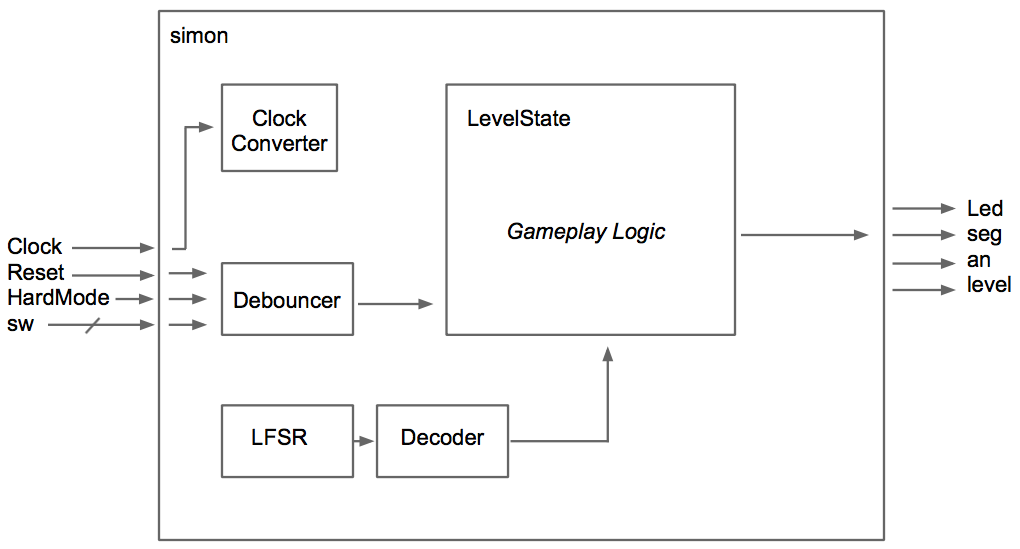
\includegraphics[width=\textwidth]{highLevel.png}
\caption{A high level diagram of our Simon game.}
\label{fig:high}
\end{figure}

As can be seen in the figure above, our top-level module accepts two main user inputs: \texttt{HardMode}, which indicates the difficulty level the user would enjoy, and \texttt{sw}, which represents the guesses the user makes during gameplay.\\

The \texttt{Led} output flashes lights above each switch to indicate to the user which of the four switches must be flipped during the level at hand. The \texttt{level} signal maps to the remaining 4 LEDs and shows the binary representation of the current level. Lastly, the \texttt{seg} and \texttt{an} outputs serve a similar purpose, except that they output the decimal representation of the current level.

\subsection{Low Level Implementation}


\section{Simulation Documentation}

Along with simulating and testing the overall game, we modularized our code and tested each of the modules individually. \\

For the overall game, we simulated the game from level one through level 10 and covered both correct and incorrect input. We discovered that when the user inputs an incorrect switch, the program did not produce a new random sequence but instead restarted the game using the same sequence from before. \\

Our simulation of the randomSequenceGenerator module showed that not only was our sequence "pseudo-random", it had a period of 7 numbers. We then adjusted to increase that number.

\section{Conclusion}


\end{document}

